\frame
{
	\frametitle{Genome Rearrangement Distance}
	\begin{itemize}
	\item The minimum number of operations to transform $G_1$ into $G_2$
	\end{itemize}

	\vspace{0.2cm}

	\begin{center}
		\includegraphics[width=0.6\textwidth]{Lec8-Genome-Rearrangement-Problem-figs/distance.pdf}
	\end{center}
}

\frame
{
	\frametitle{Adjacency Graph}
	\begin{center}
		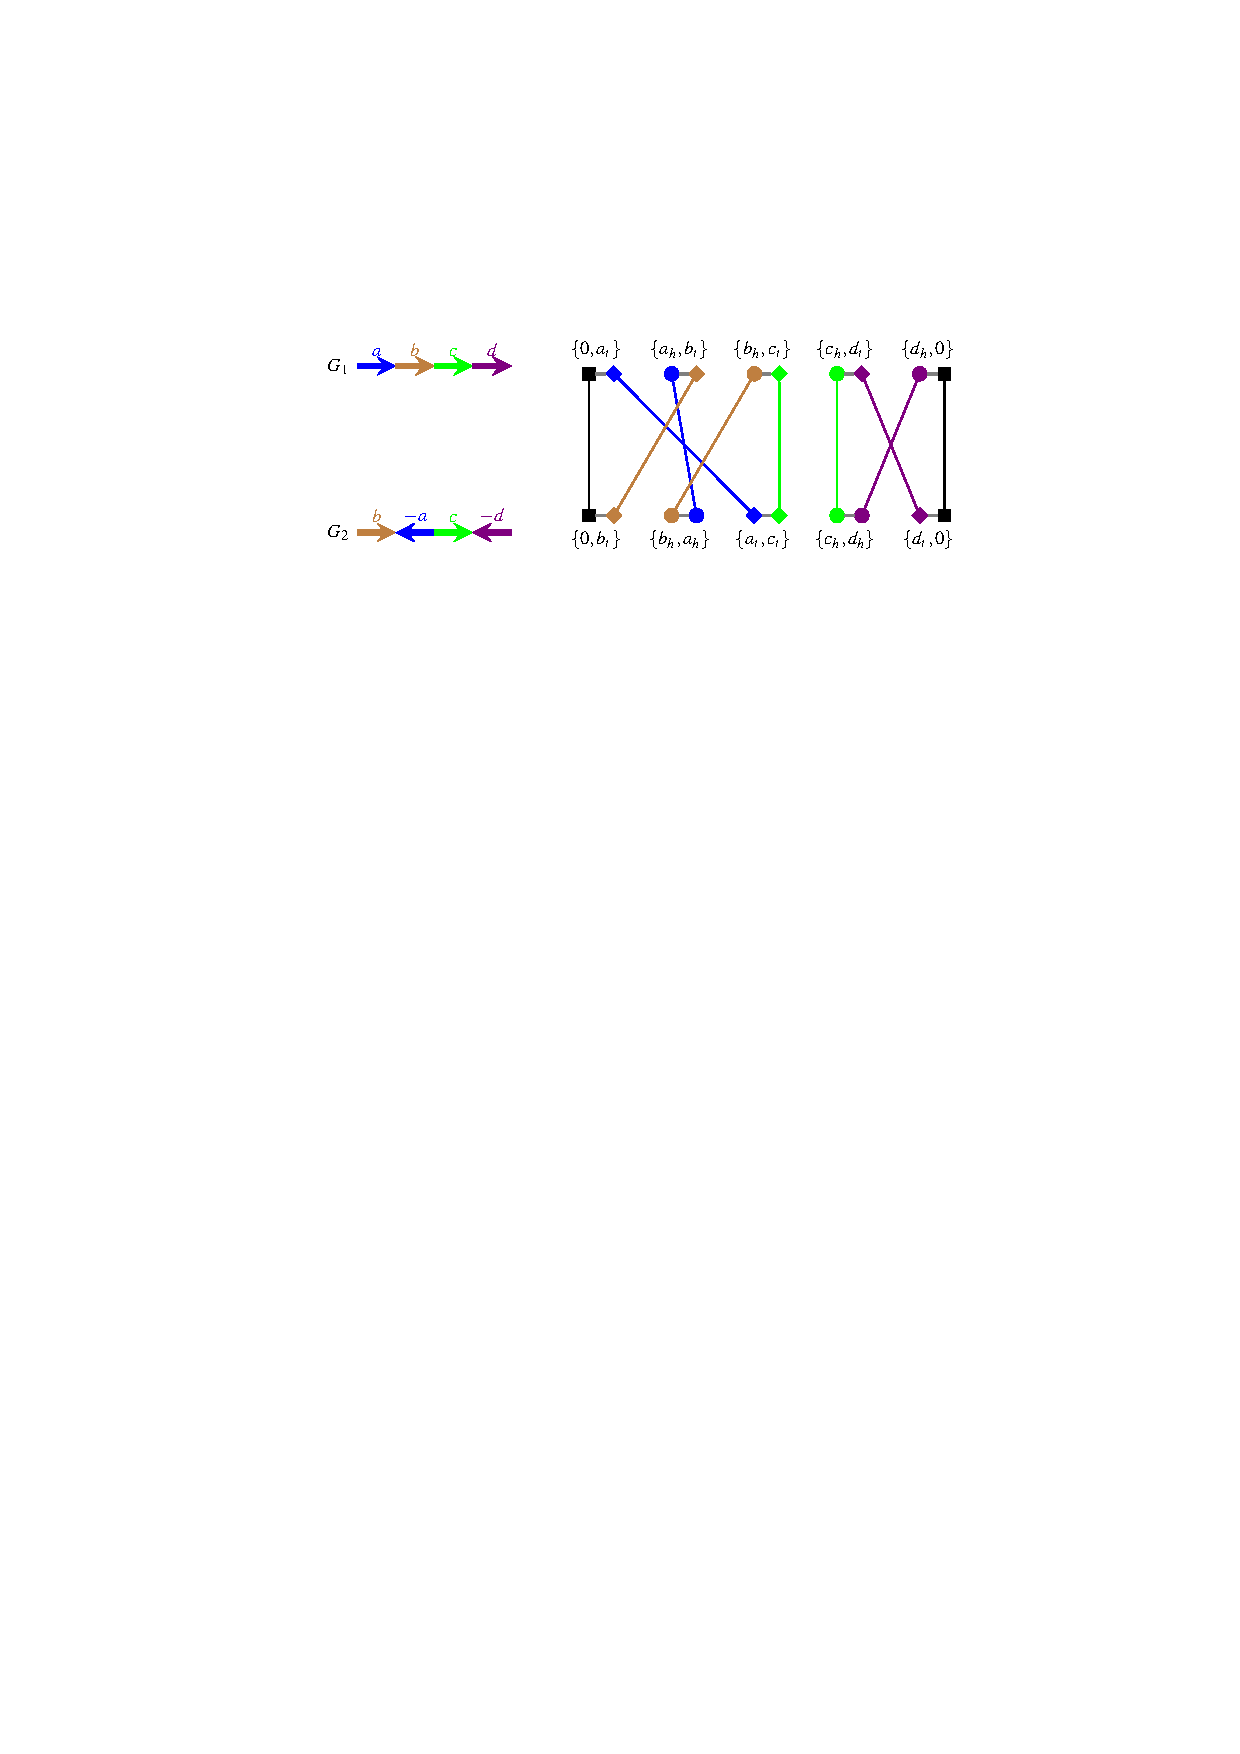
\includegraphics[width=0.95\textwidth]{Lec8-Genome-Rearrangement-Problem-figs/adjgraph.pdf}
	\end{center}
	\begin{itemize}
	\item<2-> DCJ distance = (\#adjacencies) $-$ (\#cycles).
	\item<3-> To minimize DCJ distance, we need to compute a decomposition of the corresponding
		adjacency graph with maximized number of cycles.
	\end{itemize}
}

\frame
{
	\frametitle{Problem Statement}

	\vspace{-0.3cm}	

	{\bf Problem:} given an undirected graph $G=(V,E)$, to choose $k$ edges and remove others,
	such that the number of connected components in the remaining graph is maximized. \\
	({\bf Formulate this problem as an ILP}.)

	\vspace{0.6cm}	

	\begin{center}
	\includegraphics[width=\textwidth]{Lec8-Genome-Rearrangement-Problem-figs/star.pdf}
	\end{center}
}

\frame
{
	\frametitle{ILP Formulation}

	Consider the following example with $k = 3$.

	\begin{center}
	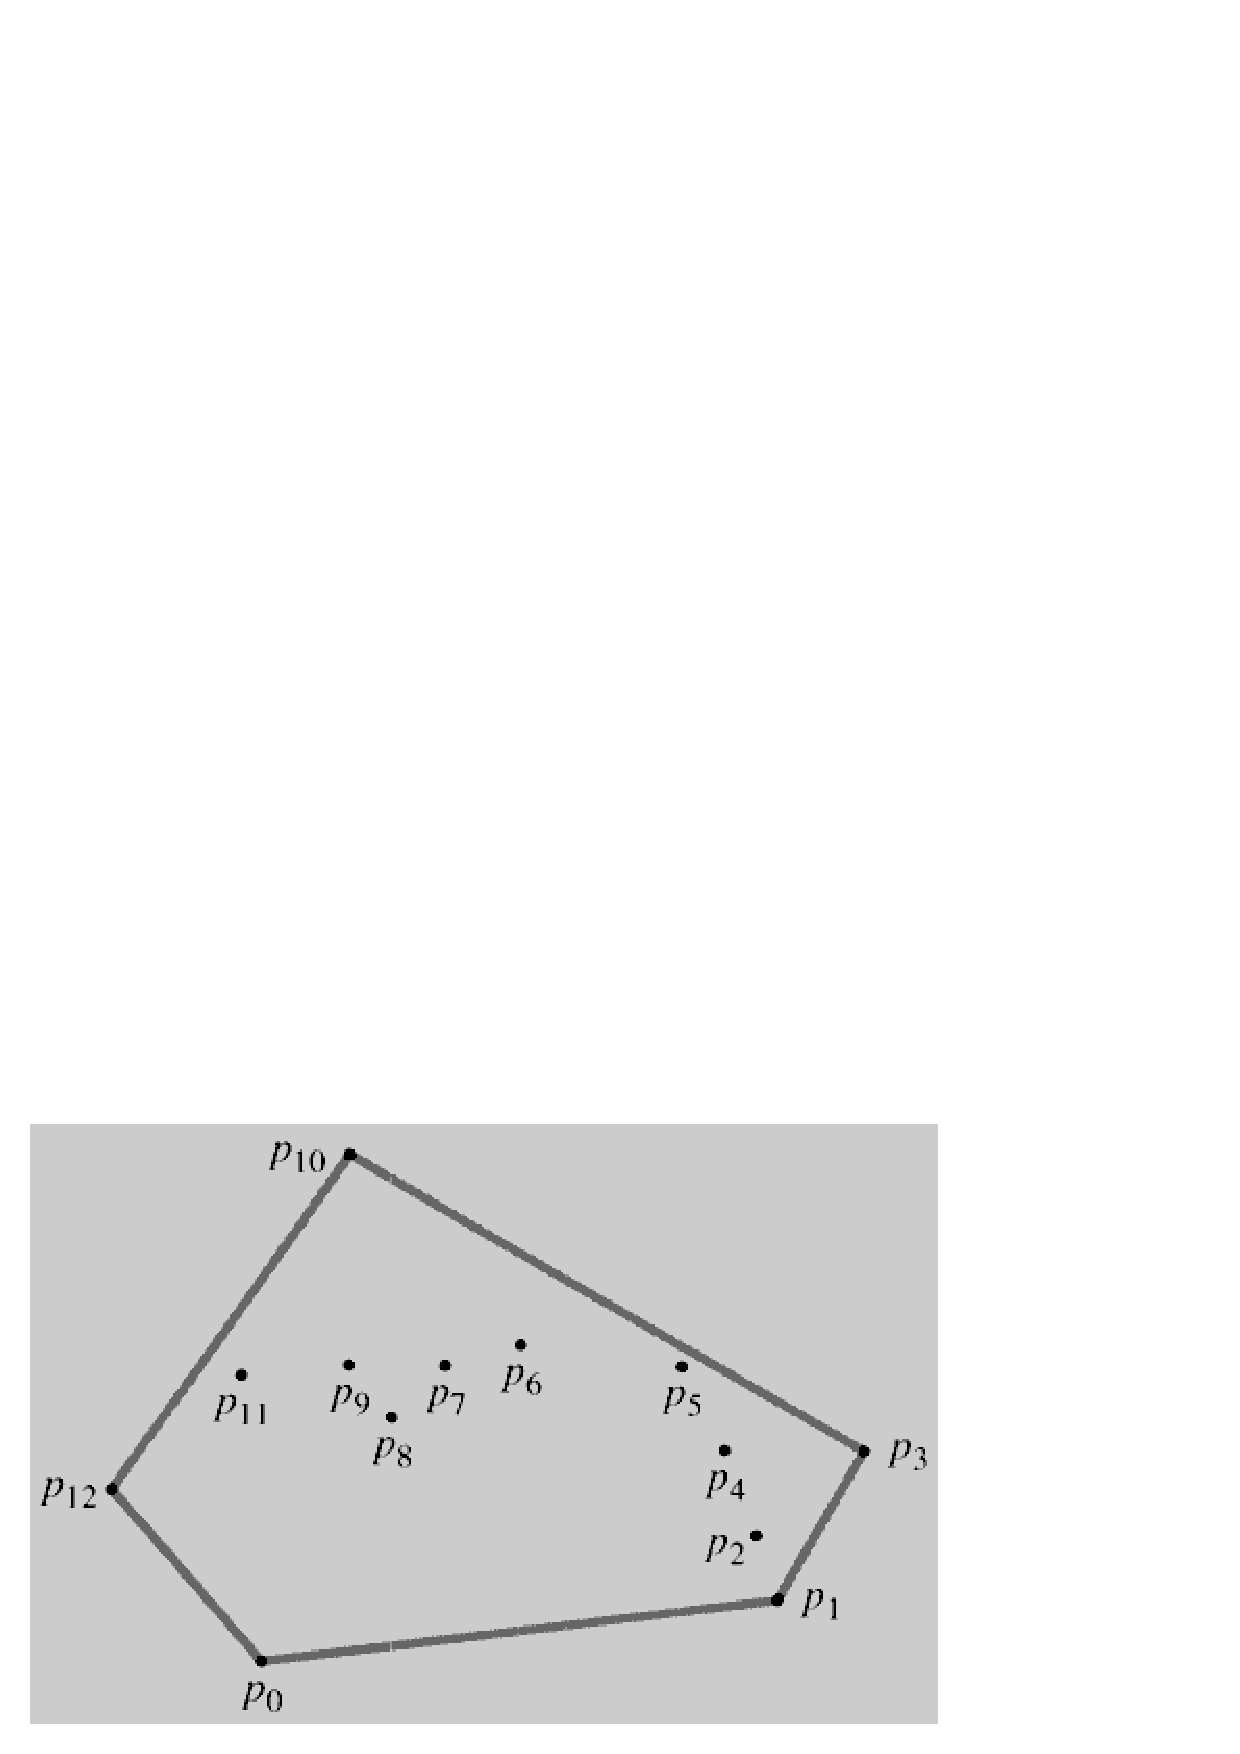
\includegraphics[width=0.5\textwidth]{Lec8-Genome-Rearrangement-Problem-figs/example.pdf}
	\end{center}

	\begin{itemize}
	\item<2-> For each edge $e_i$, we use a binary variable $x_i$ to indicate whether $e_i$ is chosen.
		We use the following constraint to guarantee exactly $k$ edges are chosen:
		\begin{displaymath}
			x_1 + x_2 + x_3 + x_4 + x_5 = 3
		\end{displaymath}
	\end{itemize}

}

\frame
{
	\frametitle{ILP Formulation}

	\begin{center}
	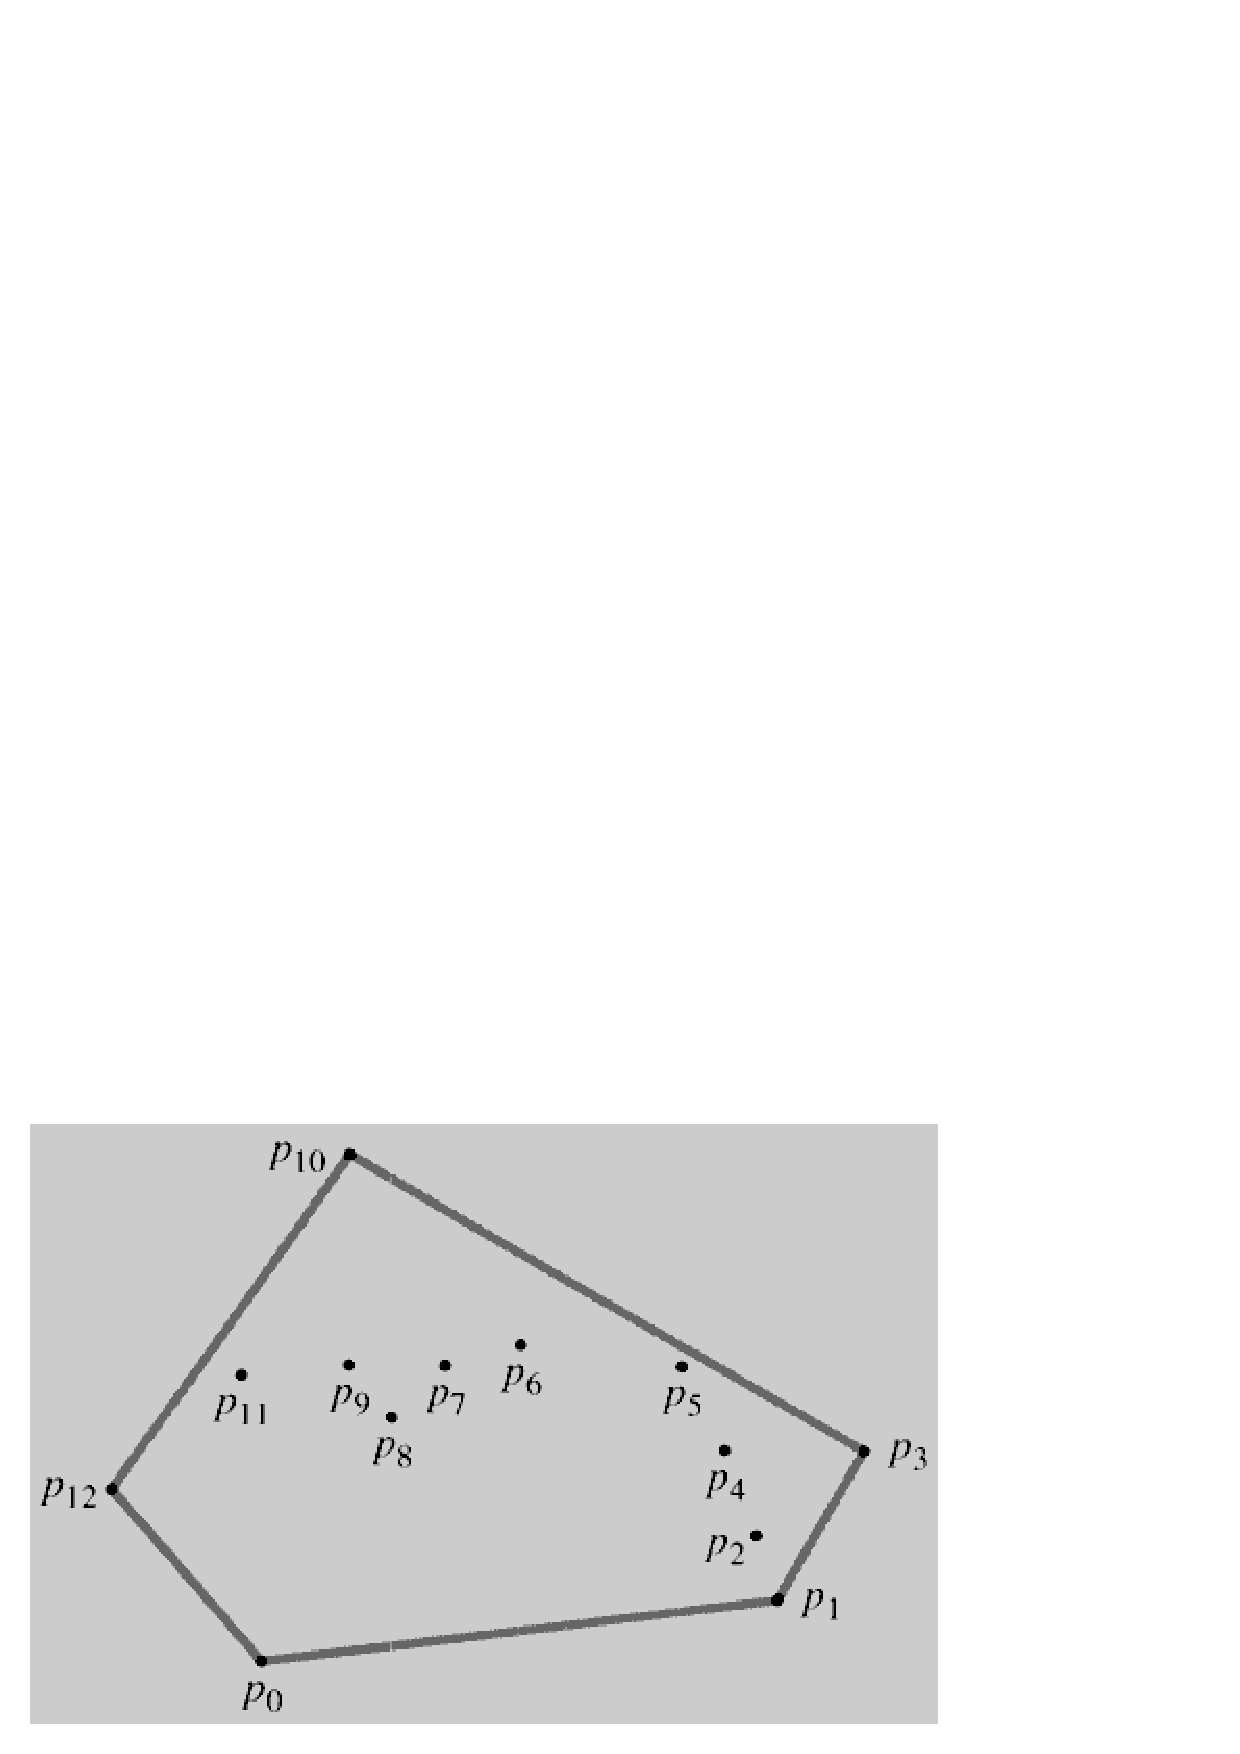
\includegraphics[width=0.5\textwidth]{Lec8-Genome-Rearrangement-Problem-figs/example.pdf}
	\end{center}


	\begin{itemize}
	\item<1-> To count the number of connected components, for vertex $v_j$, $1\le j \le |V|$,
		we use a variable $y_j$ to indicate the {\bf label} of $v_j$, and set {\bf distinct} upper 
		bounds for all the labels:
		\begin{eqnarray*}
			1\le  y_1  \le 1\\ 
			1\le  y_2  \le 2\\ 
			1\le  y_3  \le 3\\ 
			1\le  y_4  \le 4\\ 
		\end{eqnarray*}
	\end{itemize}

}

\frame
{
	\frametitle{ILP Formulation}

	\begin{center}
	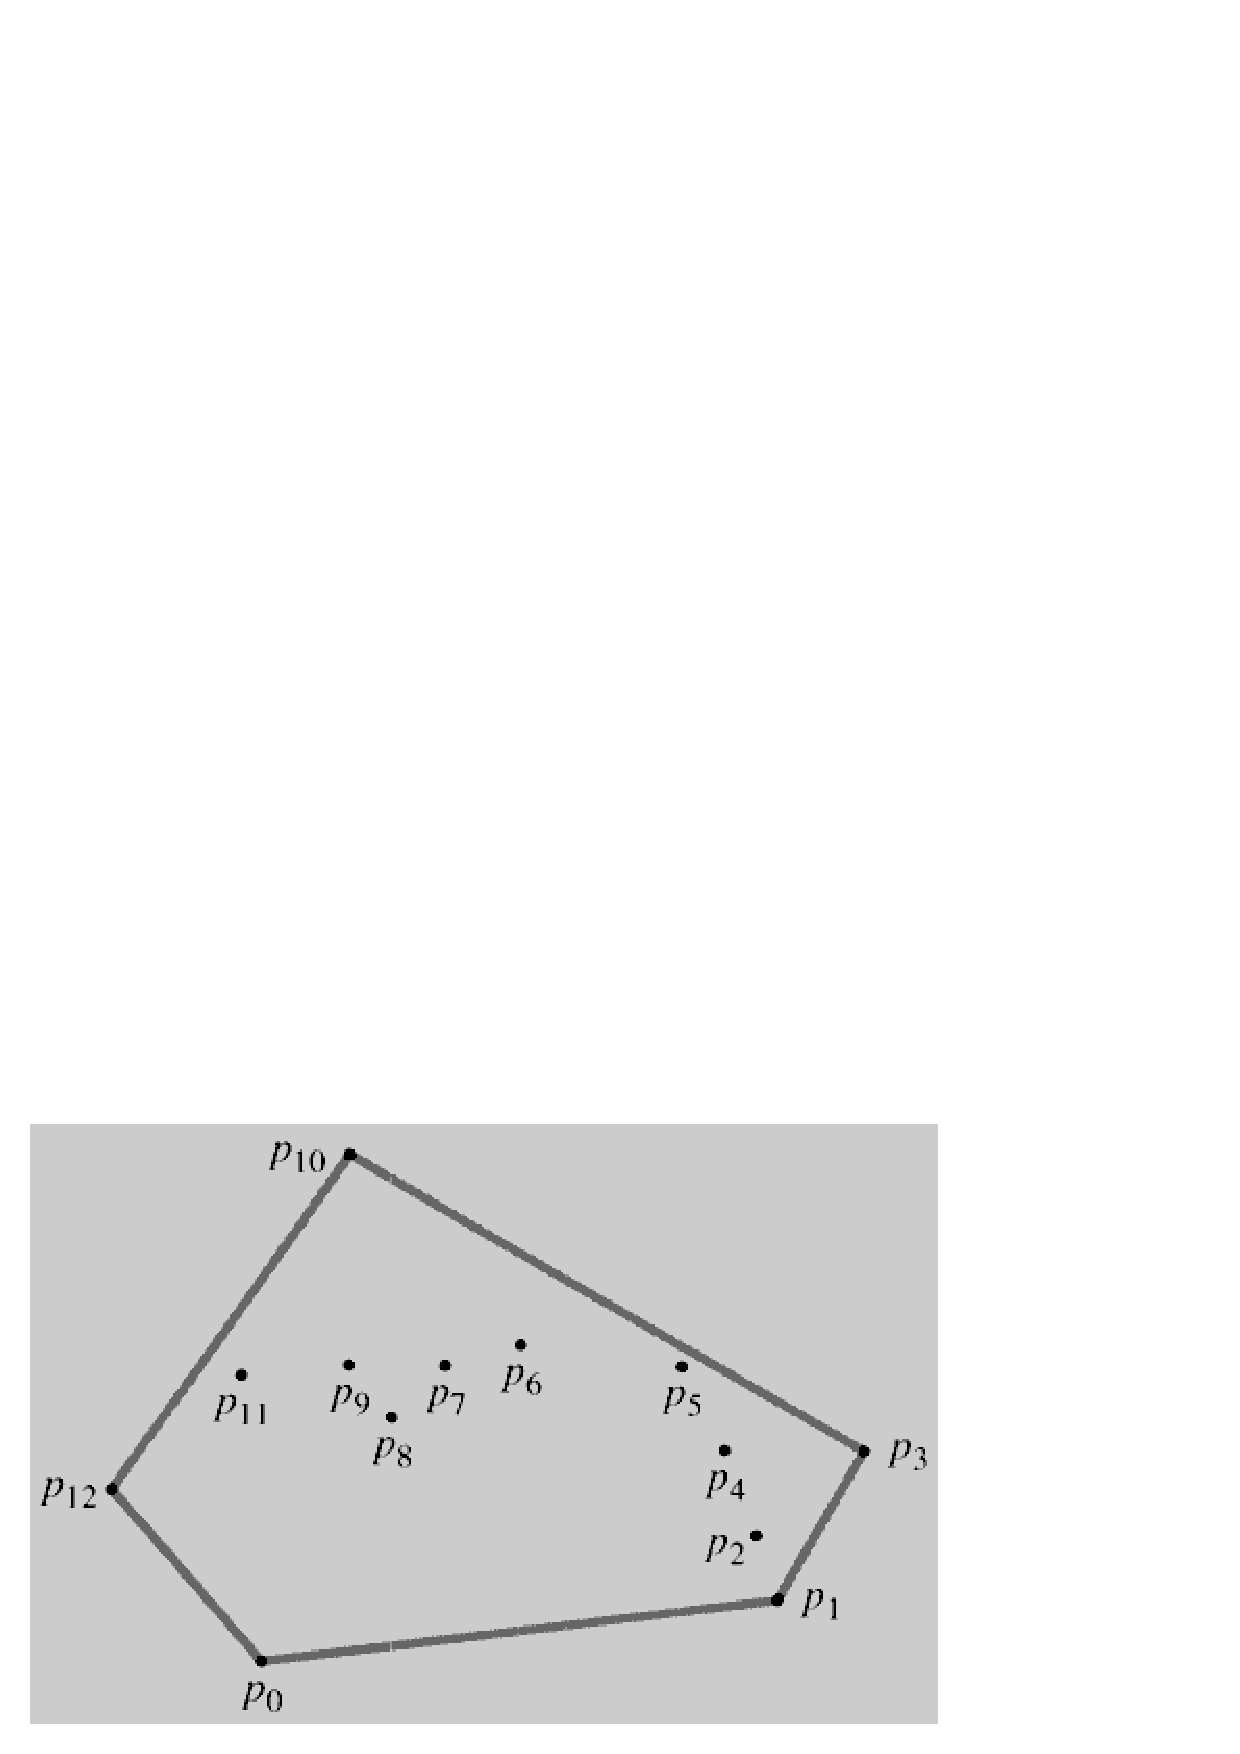
\includegraphics[width=0.5\textwidth]{Lec8-Genome-Rearrangement-Problem-figs/example.pdf}
	\end{center}

	\begin{itemize}
	\item<1-> We guarantee that if an edge is chosen, then its two adjacent vertices have the same label: 
		\begin{align*}
			y_1 \le y_2 + 1 \cdot (1 - x_1);\  y_2 \le y_1 + 2 \cdot (1 - x_1) \tag{for $e_1$}\\
			y_1 \le y_3 + 1 \cdot (1 - x_2);\  y_3 \le y_1 + 3 \cdot (1 - x_2) \tag{for $e_2$}\\
			y_2 \le y_3 + 2 \cdot (1 - x_3);\  y_3 \le y_2 + 3 \cdot (1 - x_3) \tag{for $e_3$}\\
			y_2 \le y_4 + 2 \cdot (1 - x_4);\  y_4 \le y_2 + 4 \cdot (1 - x_4) \tag{for $e_4$}\\
			y_3 \le y_4 + 3 \cdot (1 - x_5);\  y_4 \le y_3 + 4 \cdot (1 - x_5) \tag{for $e_5$}\\
		\end{align*}
	\end{itemize}
}

\frame
{
	\frametitle{ILP Formulation}

	\begin{center}
	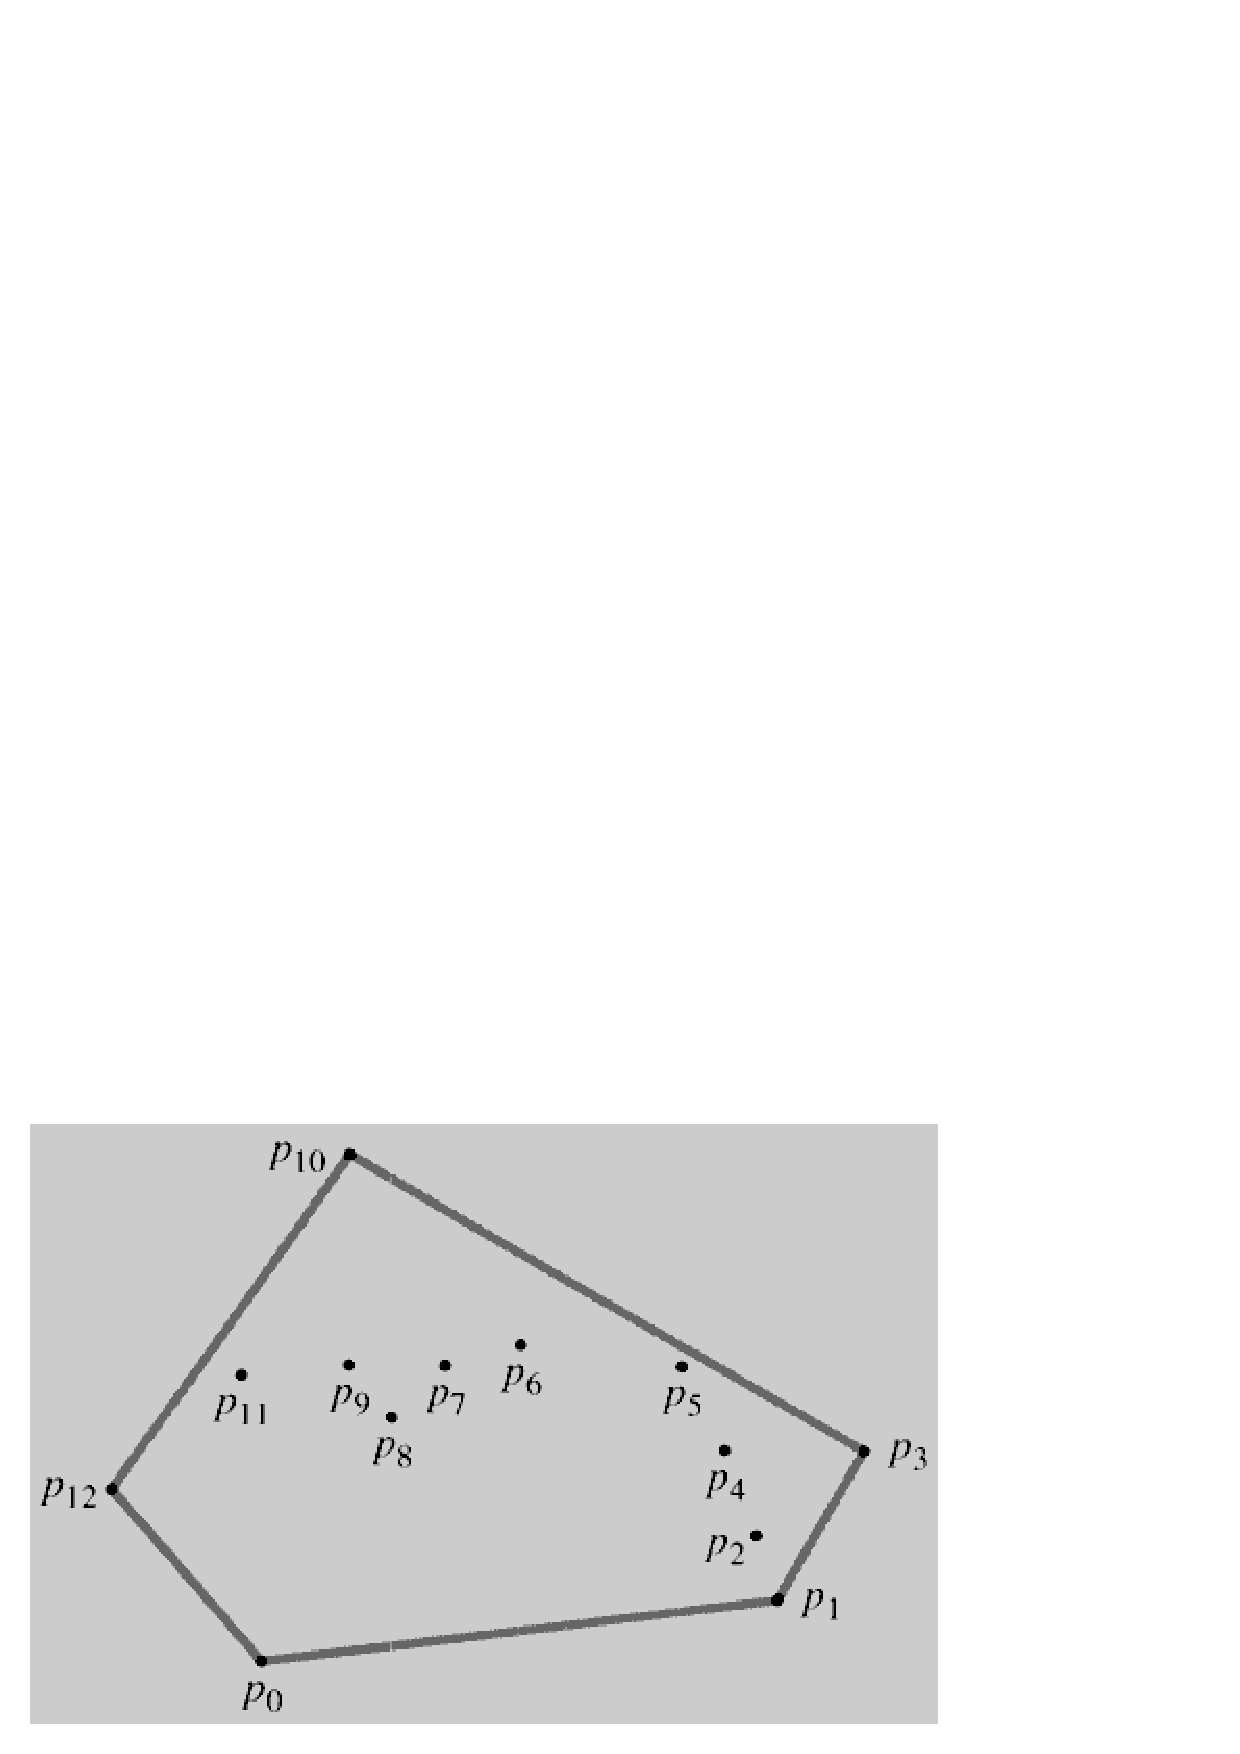
\includegraphics[width=0.5\textwidth]{Lec8-Genome-Rearrangement-Problem-figs/example.pdf}
	\end{center}

	\begin{itemize}
	\item<2-> The equality can propagate along the chosen edges. Thus, in the remaining graph
		all vertices in the same connected component have the same label.

	\item<3-> Since all vertices have distinct upper bounds, in each connected
	component, at most one vertex can reach its upper bound. Thus, we
	can use the number of vertices whose upper bound is reached, to count the number of connected components.

	\end{itemize}
}


\frame
{
	\frametitle{ILP Formulation}

	\begin{center}
	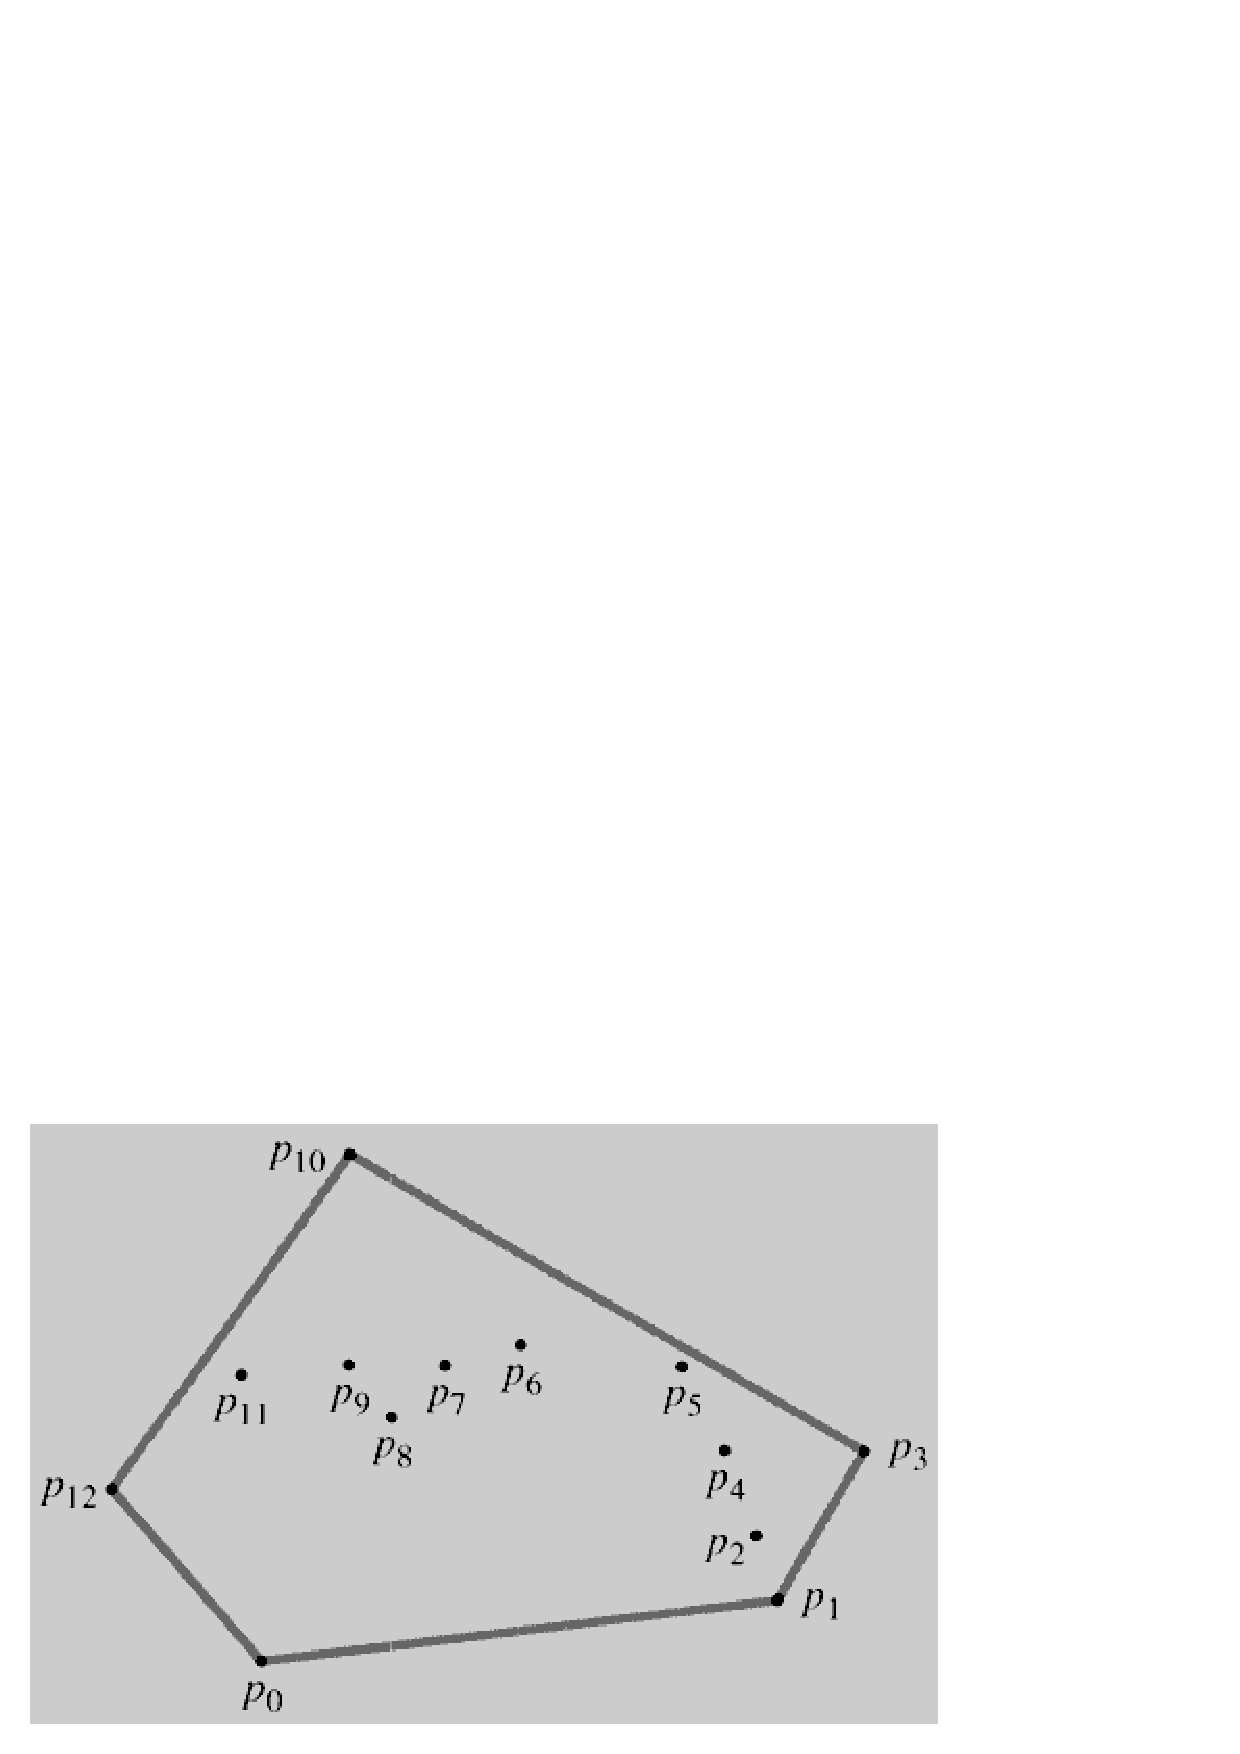
\includegraphics[width=0.5\textwidth]{Lec8-Genome-Rearrangement-Problem-figs/example.pdf}
	\end{center}

	\begin{itemize}
	\item<2-> We use a binary variable $z_j$ to indicate whether the label of $v_j$ reaches its upper bound:
		\begin{eqnarray*}
			1 \cdot z_1 \le y_1 \\
			2 \cdot z_2 \le y_2 \\
			3 \cdot z_3 \le y_3 \\
			4 \cdot z_4 \le y_4 
		\end{eqnarray*}
	We can verify that, $z_j = 1$ only if $y_j = j$, i.e., the label of $v_j$ reaches its upper bound.
	\end{itemize}
}


\frame
{
	\frametitle{ILP Formulation}

	\begin{center}
	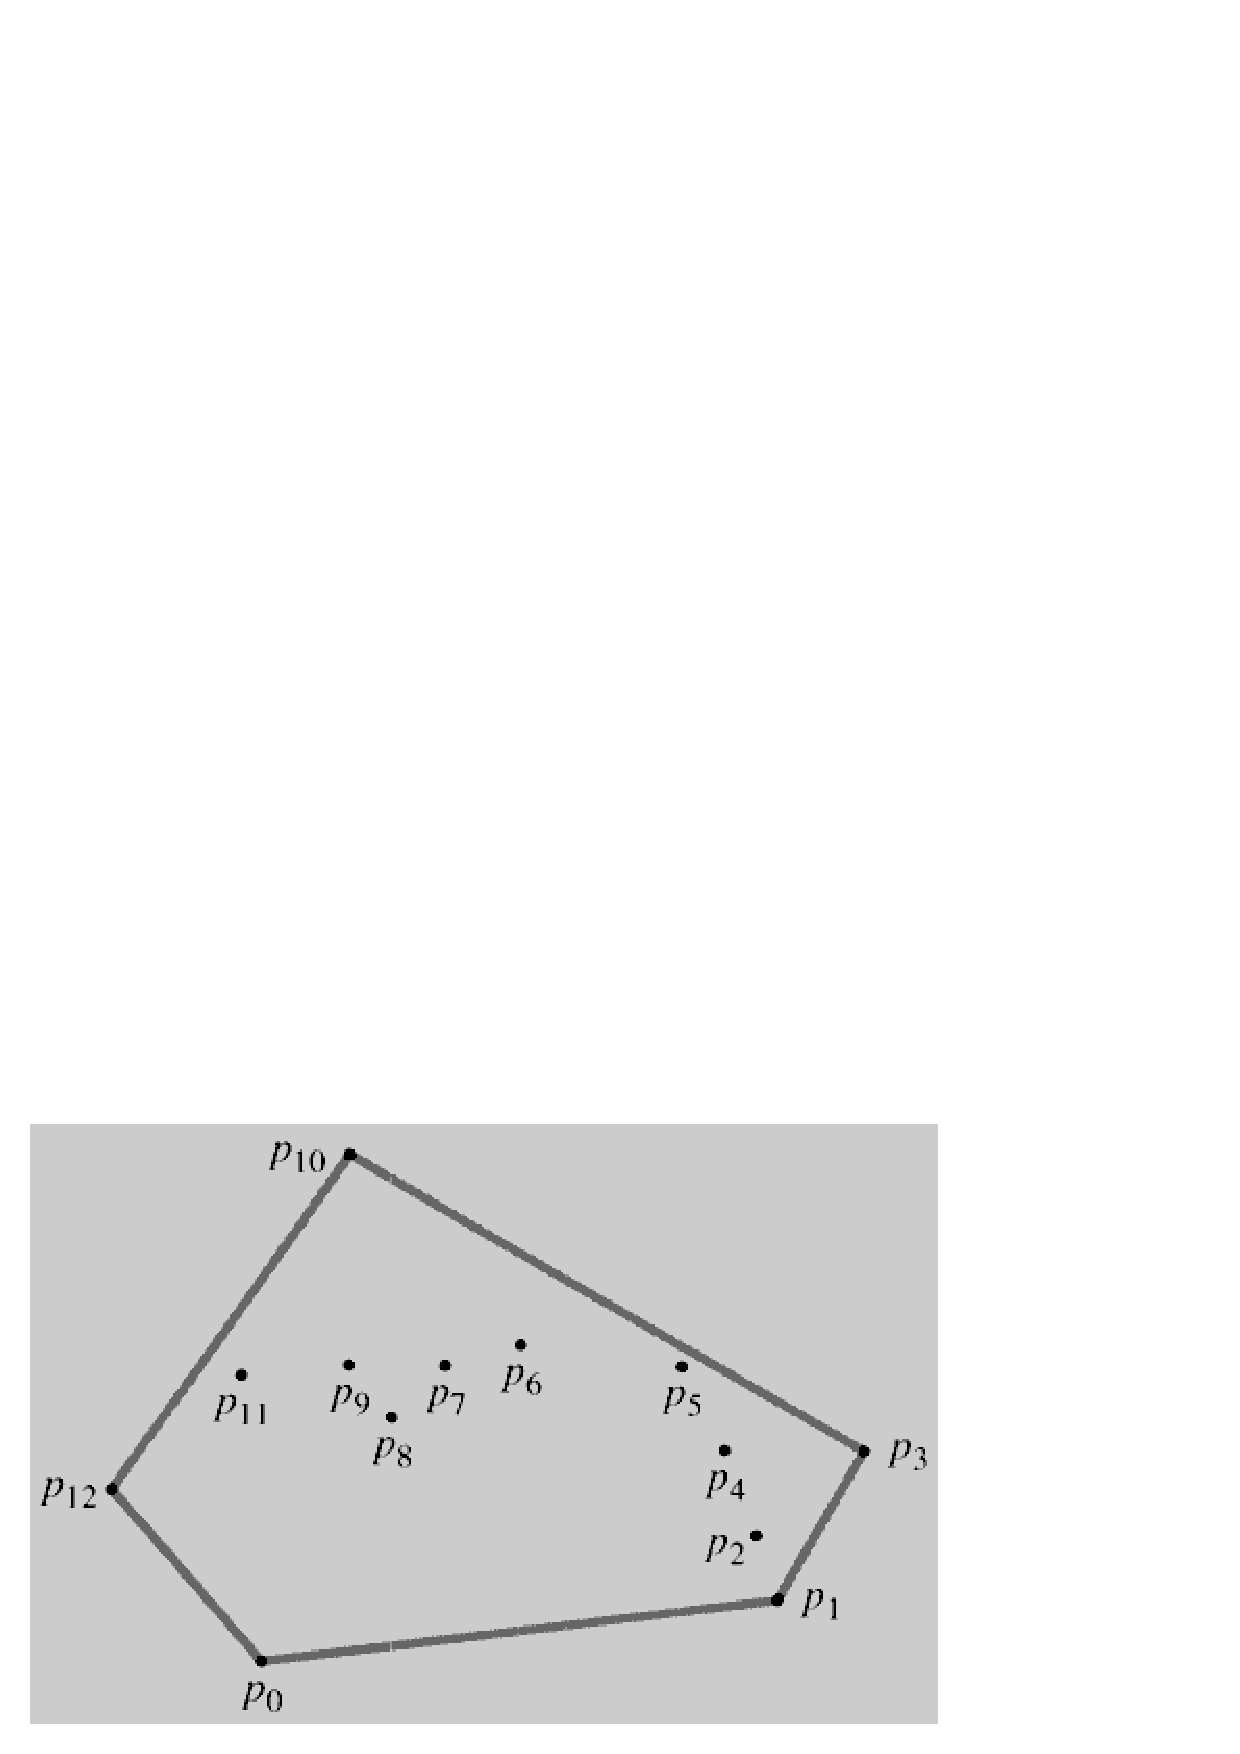
\includegraphics[width=0.5\textwidth]{Lec8-Genome-Rearrangement-Problem-figs/example.pdf}
	\end{center}

	\begin{itemize}
	\item<2-> The objective function of the ILP formulation can be set to maximize the number of vertices
		whose upper bound can be reached:
		\begin{displaymath}
			\max z_1 + z_2 + z_3 + z_4
		\end{displaymath}
	\end{itemize}
}
